\documentclass[slovak,a4paper,10pt]{article}

\usepackage[utf8]{inputenc}
\usepackage{graphicx}
\usepackage{booktabs}
\usepackage{array}
\usepackage{paralist}
\usepackage{verbatim}
\usepackage{subfig}
\usepackage{amsmath}
\usepackage{index}
\usepackage{cite}
\usepackage[slovak]{babel}
\usepackage{fancyhdr}
\pagestyle{fancy}

\usepackage{sectsty}
\allsectionsfont{\sffamily\mdseries\upshape}

\usepackage[nottoc,notlof,notlot]{tocbibind}
\usepackage[titles,subfigure]{tocloft}
\renewcommand{\cftsecfont}{\rmfamily\mdseries\upshape}
\renewcommand{\cftsecpagefont}{\rmfamily\mdseries\upshape}

\title{Počítačové hry, ktoré učia programovať}
\author{Samuel Suja\\
	{\small Slovenská technická univerzita v Bratislave}\\
	{\small Fakulta informatiky a informačných technológií}\\
	{\small \texttt{xsujas@stuba.sk}}
}
\date{13.12.2020}

%

\begin{document}
\maketitle

\begin{abstract}

Online vyučovanie sa v súčasnej situácií stalo nenahraditeľnou súčasťou študentského života. Niekedy však vedomosti zo školy nestačia na to, aby študenti vedeli všetko, čo potrebujú. V takom prípade je najlepšou možnosťou samoštúdium. Jednou z metód samoučenia je aj hranie počítačových hier. Napriek tomu že ich veľa ľudí berie ako stratu času, počítačové hry nás dokážu naučiť veci ako cudzie jazyky, logiku, históriu, a podobne. V tomto článku sa budeme venovať konkrétne takým počítačovým hrám, ktoré nás dokážu naučiť programovať, alebo nám aspoň vysvetliť základné princípy programovania. Zameriame sa na hry, ktoré sú založené na vykonávaní úloh pomocou písania alebo zoraďovania kódu, alebo ktoré obsahujú prvkypodobné samotnému programovaniu. Tými hrami budú ToonTalk, LightBot, LeekWars a CodinGame, ktoré vedia pomôcť programátorom v rôznych oblastiach ich profesie.

\end{abstract}

%Úvod
\section{Úvod}
Hry umožňujú hráčom zažiť, vyskúšať, alebo sa naučiť rôzne zručnosti, a zároveň sa pri tom zabávať \cite{burgos2007re}. Pomocou hier môžeme študentom ukázať nové riešenia problémov zábavným, ale zároveň efektívnym spôsobom. Pre študentov, ktorí majú problémy s pochopením niektorých tém v škole, môžu práve počítačové hry poskytnúť nový pohľad na učivo, a v niektorých prípadoch byť aj lepšou alternatívou pre vysvetlenie ťažšieho učiva \cite{seng2014computer}. V tomto článku sa bližšie pozreme na hry ktoré dokážu ľudí naučiť programovať, riešiť logické problémy, alebo pracovať s umelou inteligenciou; konkrétne hry ToonTalk, LightBot, LeekWars a CodinGame.

%ToonTalk
\section{ToonTalk}
ToonTalk je programovací jazyk, ktorého kód môžeme vidieť v podobe interaktívneho animovaného sveta \cite{kahn1999computer}. K dispozícií máme prázdne pole a niekoľko objektov, ktoré je možné na pole umiestniť a vytvoriť funkčný program. Animované nie sú len ikony týchto objektov, ale aj samotné činnosti ktoré vykonávajú (Obr. \ref{fig:obr1}). Vďaka tomu môže použivateľ v reálnom čase sledovať ako jeho program pracuje.
\paragraph{Reakcia na prednášku 4:}
Raz vidieť je lepšie ako stokrát počuť. Vďaka animovanému prostrediu môže ToonTalk vysvetliť základy programovania aj ľuďom, ktorí nevedia pochopiť ako funguje kód ich programu. Týmto zároveň prepája programovací svet s umeleckým, čím umožňuje vznik nových nápadov.
\begin{figure}[h]
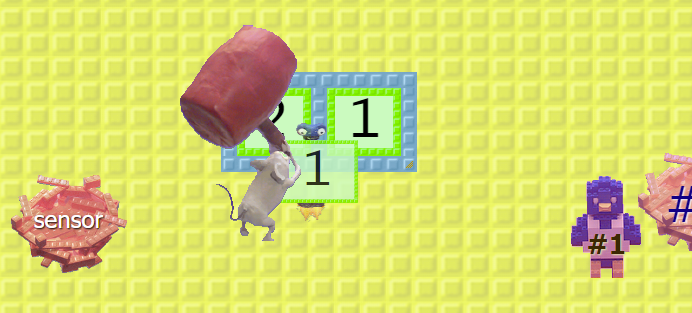
\includegraphics[scale=0.4]{toontalkmain}
\centering
\caption{ToonTalk v akcii: Myš zvyšuje číslo o 1}
\label{fig:obr1}
\end{figure}
\subsection{Priebeh hry}
Základom ToonTalku sú samotné objekty, ktoré zastupujú príkazy a funkcie štandardných programovacích jazykov. Medzi ne patria:
\begin{center}
\begin{tabular}{|c|c|c|}
\hline
Názov & Anglický názov & Funkcia \\
\hline
Čísla & Numbers & Vstupy do aritmetických operácií \\
\hline
Škatule & Boxes & Ukladanie objektov \\
\hline
Vtáky a hniezda & Birds and nests & Posielanie správ \\
\hline
Váhy & Scales & Porovnávanie objektov a hodnôt \\
\hline
Senzory & Sensors & Rozpoznávanie kliknutí a kláves \\
\hline
Funkčné vtáky & Function birds & Vykonávanie funkcii \\
\hline
Roboti & Robots & Učenie sa vykonávať prácu \\
\hline
Prehliadačové prvky & Browser elements & Práca s obsahom stránok \\
\hline
\end{tabular}
\end{center}
\begin{figure}[h]
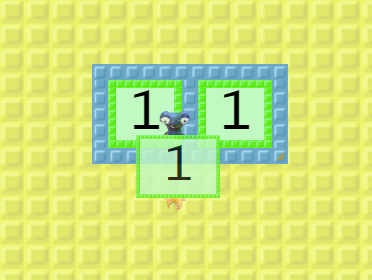
\includegraphics[scale=0.5]{toontalkrobot}
\centering
\caption{Robot naprogramovaný na to, aby pripočítaval 1 k číslu v škatuli naľavo}
\label{fig:obr2}
\end{figure}

%LightBot
\section{LightBot}
LightBot nie je hra, ktorá dokáže hráčom priamo vysvetliť princípy programovania. Jadro tejto hry spočíva v skladaní príkazov do algoritmov s cieľom dostať sa do ďalšej úrovne \cite{combefis2016learning}. V hre ovláda hráč robota, ktorý sa vie pohybovať po políčkach a vykonávať rôzne úlohy. Aby hráč postúpil do ďalšej úrovne, musí pomôcť robotovi zapáliť svetlá na všetkých políčkach zafarbených modrou farbou (Obr. \ref{fig:obr3}). Toto hráč docieli poskladaním postupnosti príkazov do procedúry main, ktoré má robot vykonať aby úspešne dokončil úroveň.
\paragraph{Reakcia na prednášku 8:}
LightBot umožňuje hráčom hľadať svoje vlastné riešenia pre zadané problémy, čím zlepšuje ich originalitu a kreatívne myslenie. To môže byť prepojené aj s činnosťami ako napríklad tvorba článkov a prezentácií, pretože bude pre nich ľahšie vyhnúť sa plagiátorstvu.
\begin{figure}[h]
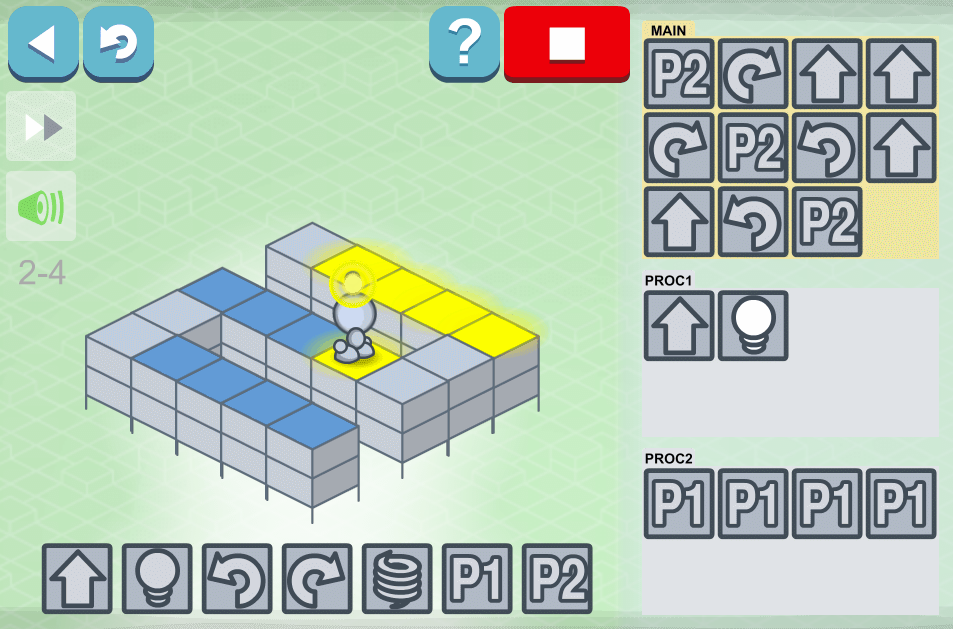
\includegraphics[scale=0.3]{lightbotmain}
\centering
\caption{Úspešné riešenie úrovne 2-4}
\label{fig:obr3}
\end{figure}
\subsection{Priebeh hry}
Na pravej strane obrazovky sa nachádza procedúra main: po stlačení tlačidla na spustenie robota vykoná LightBot príkazy zadané v tejto funkcií. Main má limit 12 príkazov, čo núti hráča byť čo najefektívnejším. V neskorších úrovniach pribudnú ďalšie procedúry, ktoré môžeme opakovane vykonať cez procedúru main. \\
Na dolnej strane obrazovky sa nachádzaju samotné príkazy, ktoré môže robot vykonať. Medzi ne patrí:
\begin{itemize}
\item Pohyb dopredu
\item Zapálenie alebo zhasnutie svetla na políčku
\item Otočenie doľava
\item Otočenie doprava
\item Skok - špeciálny pohyb dopredu, ktorým sa dá pohybovať medzi políčkami rôznych výšok
\item Procedúra - vykoná všetky príkazy vo vybranej procedúre
\end{itemize}

%LeekWars
\section{LeekWars}
LeekWars je online hra pre viac hráčov, v ktorej hráč bojuje so svojim pórom (ang. leek) proti pórom ostatných hráčov (Obr. \ref{fig:obr4}) \cite{combefis2016learning}. Hráč môže pre svoj pór kupovať rôzne zbrane a čipy, ktoré mu pridávajú nové schopnosti, alebo mu zlepšovať jeho štatistiky (napr. rýchlosť, životy, sila). Bojovaním zvyšuje pór svoju úroveň a stáva sa silnejším. Póru však môže dávať príkazy len kód, ktorý mu hráč napíše pred tým, ako ho pošle do boja.
\begin{figure}[h]
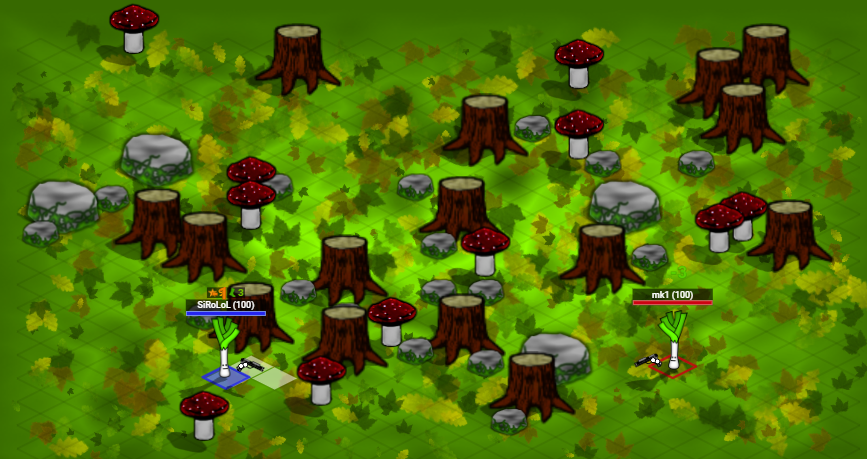
\includegraphics[scale=0.3]{leekwarsmain}
\centering
\caption{Pór hráča (vľavo) bojuje proti póru iného hráča (vpravo)}
\label{fig:obr4}
\end{figure}
\begin{figure}[h]
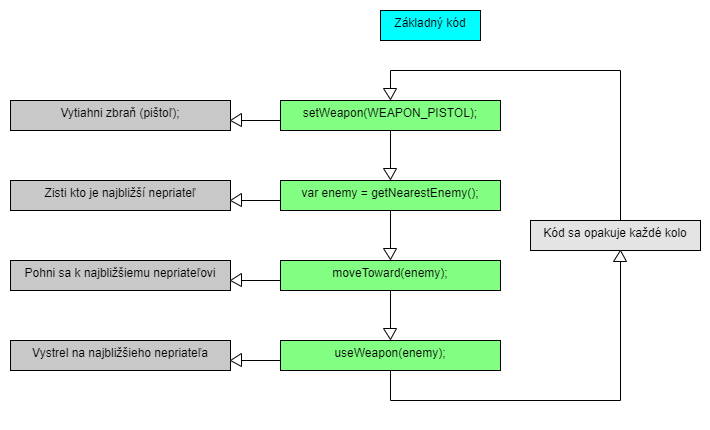
\includegraphics[scale=0.4]{leekwarscode}
\centering
\caption{Základný kód, ktorý hráč dostane na prvej úrovni}
\label{fig:obr5}
\end{figure}
\subsection{Priebeh hry}
Hráč si najprv vytvorí svoj pór, ktorý začína na prvej úrovni. Ku svojmu póru dostane základný kód (Obr.~\ref{fig:obr5}), ktorý môže už od začiatku upraviť v editore kódu. Ďalej má hráč sprístupnený trh (ang. Market), kde si môže nakúpiť nové zbrane a čipy. Herné peniaze aj body skúsenosti potrebné na nákup nových zbraní môže hráč získať v záhrade (ang. Garden), kde bojuje proti iným hráčom. \\
Samotný boj spočíva v striedaní pohybov hráčov po kolách. Boj sa končí keď má jeden z hráčov 0 životov, alebo keď vyprší čas. Po skončení boja dostávajú obaja hráči body skúseností a herné peniaze.

%CodinGame
\section{CodinGame}
CodinGame je online hra, v ktorej je hráčovým cieľom naprogramovať svojho agenta tak, aby splnil požiadavky na prejdenie úrovňou \cite{combefis2016learning}. Hráč si môže vybrať jeden z dostupných jazykov, v ktorom bude programovať, a napíše svoj kód tak, aby jeho agent úspešne prešiel cez všetky testovacie situácie. Každá testovacia situácia vloží agenta do iných podmienok, ale hráč musí pre všetky testovacie situácie použiť ten istý kód. Podmienky niektorých z týchto testov sú hráčovi predom známe, no niektoré sú skryté, aby hráč dospel k všeobecnému riešeniu.\\
\begin{figure}[h]
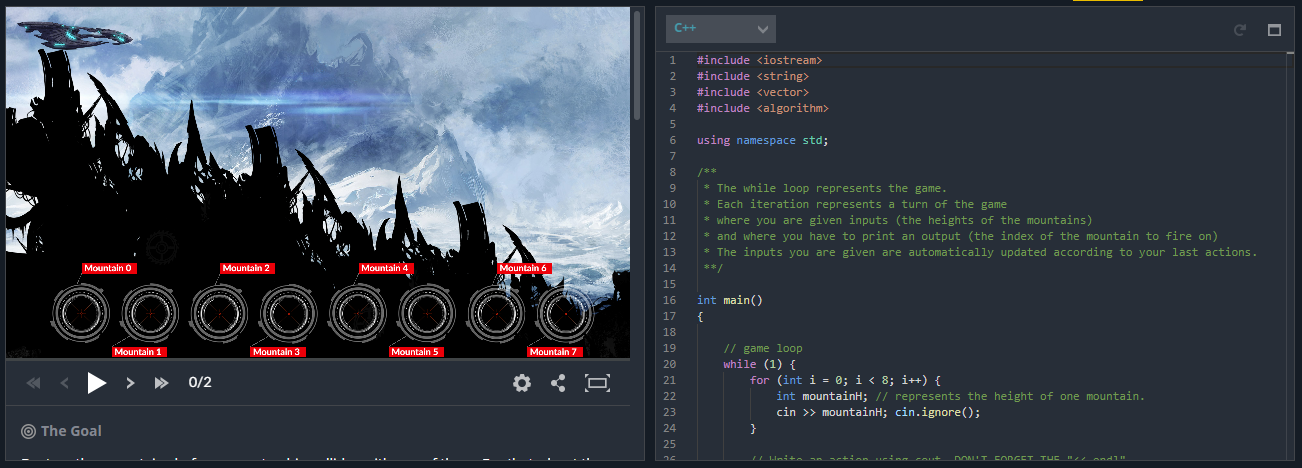
\includegraphics[scale=0.28]{codingamemain}
\centering
\caption{Začiatočnícka úroveň "The Descent". Na ľavej strane sa nachádza úroveň, ktorej cieľom je zničiť s loďou všetky hory bez toho, aby do nich loď narazila}
\label{fig:obr6}
\end{figure}
\subsection{Priebeh hry}
Na začiatku si hráč vyberie jednu z dostupných úrovní, ktoré sú rozdelené podľa obtiažnosti. Po spustení sa na obrazovke objaví okno s kódom, okno pre výber jednej z testovacích situácii, a okno so samotnou úrovňou (Obr. \ref{fig:obr6}). Hráčovi je v kóde pomocou komentárov vysvetlené, čo kód robí, a hráč môže ďalej k riešeniu pristupovať akýmkoľvek spôsobom. Na obrazovke vidí hráč svojho agenta a prostredie, v ktorom sa nachádza. Hráč si ďalej môže svoj kód spustiť len v jednej z testovacích situácií, alebo ho môže naraz spustiť vo všetkých. Ak hráč úspešne splní podmienky dokončenia v každej testovacej situácií, úroveň je úspešne dokončená a hráč je odmenený bodmi skúseností.\\
\paragraph{Reakcia na prednášku 2:}
Cez stránku CodinGame si môžu použivatelia nájsť prácu vo firmách ako Google a Microsoft, alebo sa zúčastniť rôznych kurzov ktoré ich naučia ako správne vykonávať inžiniersku prácu. Medzi týmito kurzami sa nachádza aj kurz práce s nástrojmi Git a GitHub, alebo rôznymi programovacími jazykmi. Ak sa ich však použivatelia nechcú zúčastniť, stále môžu komunikovať s inými hráčmi CodinGame na rôznych fórach.


%Záver
\section{Záver}
Videohry sa v dnešnej dobe stali pevnou súčasťou novodobej kultúry, a podľa niektorých sú rovnako významné ako televízia, filmy alebo knihy \cite{muratet2009towards}. Aj kvôli tomu môžu hry byť výborným nástrojom pre dištančné štúdium, alebo aj samoštúdium. Vďaka hrám, ktoré boli spomenuté v tomto článku, sa môžu ľudia popri hraní naučiť práve veci potrebné pri programovaní. Tými sú napríklad rôzne algoritmy, logické myslenie, alebo schopnosť riešiť problémy. Nemusia to byť však len hry opísané v tomto článku, ale aj komerčné hry, ktoré často obsahujú náučné prvky \cite{barr2018student}. Práve kvôli týmto dôvodom by mohli počítačové hry byť použité ako alternatíva k učeniu programovania, a pri správnom výbere by mohlo takéto vyučovanie byť oveľa efektívnejšie.

\bibliography{referencie}
\bibliographystyle{plain}

\end{document}
